To visualize the scenario when a network device is added or removed, Figure \ref{Figure:NetworkBase} shows an example network. A similar network has been used in the evaluation process of the application. This network contains only one switch with IPv4 address 10.0.0.2, as well as four additional devices. While the device with IPv4 address 10.0.0.1 holds the application, the other devices do not have a task related to the network discovery. Every device on this network has an SNMP daemon running and only the switch and the application device have configured traps. These traps will notify the application if a connection changes.

The scenario of removing a device from the network can be seen in Figure \ref{Figure:NetworkDeviceRemove}. Here, the connection between the switch and the device with IPv4 10.0.0.4 got removed. Because of that, the switch will send a trap to the application. The application parses the received trap and initializes an SNMP scan of the switch. The received scan indicates that the device with IPv4 10.0.0.4 got removed and it will be removed from the internal database.

In Figure \ref{Figure:NetworkDeviceAdded} the event of adding a device can be seen. For this case, a new device with IPv4 10.0.0.6 got added to the figure and a connection between it and the switch got added. The switch detects the connection and sends a trap to the application. The application initializes an SNMP scan of the switch. After parsing the result of the scan, the application detects that a new device got added to the network. It will now make an SNMP scan of the device with the IPv4 10.0.0.6 and add it and the new information of the switch to the database.

\begin{figure}
\begin{center}
    \tikzset{every picture/.style={line width=0.75pt}} %set default line width to 0.75pt        
    
    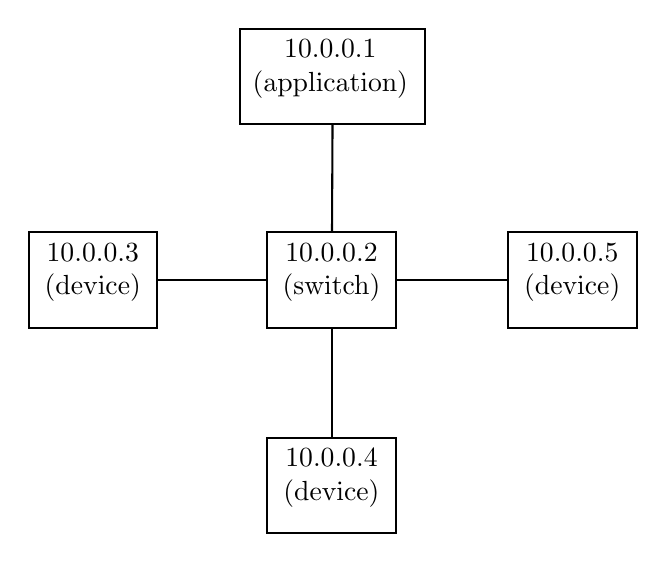
\begin{tikzpicture}[x=0.75pt,y=0.75pt,yscale=-1,xscale=1]
    %uncomment if require: \path (0,271); %set diagram left start at 0, and has height of 271
    % Text Node
    \draw    (114,11) -- (203,11) -- (203,57) -- (114,57) -- cycle  ;
    \draw (117,15) node [anchor=north west][inner sep=0.75pt]   [align=left] {\begin{minipage}[lt]{58.25pt}\setlength\topsep{0pt}
    \begin{center}
    10.0.0.1\\(application)
    \end{center}
    
    \end{minipage}};
    % Text Node
    \draw    (127,109) -- (189,109) -- (189,155) -- (127,155) -- cycle  ;
    \draw (130,113) node [anchor=north west][inner sep=0.75pt]   [align=left] {\begin{minipage}[lt]{39.55pt}\setlength\topsep{0pt}
    \begin{center}
    10.0.0.2\\(switch)
    \end{center}
    
    \end{minipage}};
    % Text Node
    \draw    (12,109) -- (74,109) -- (74,155) -- (12,155) -- cycle  ;
    \draw (15,113) node [anchor=north west][inner sep=0.75pt]   [align=left] {\begin{minipage}[lt]{39.55pt}\setlength\topsep{0pt}
    \begin{center}
    10.0.0.3\\(device)
    \end{center}
    
    \end{minipage}};
    % Text Node
    \draw    (127,208) -- (189,208) -- (189,254) -- (127,254) -- cycle  ;
    \draw (130,212) node [anchor=north west][inner sep=0.75pt]   [align=left] {\begin{minipage}[lt]{39.55pt}\setlength\topsep{0pt}
    \begin{center}
    10.0.0.4\\(device)
    \end{center}
    
    \end{minipage}};
    % Text Node
    \draw    (243,109) -- (305,109) -- (305,155) -- (243,155) -- cycle  ;
    \draw (246,113) node [anchor=north west][inner sep=0.75pt]   [align=left] {\begin{minipage}[lt]{39.55pt}\setlength\topsep{0pt}
    \begin{center}
    10.0.0.5\\(device)
    \end{center}
    
    \end{minipage}};
    % Connection
    \draw    (158.38,57) -- (158.12,109) ;
    % Connection
    \draw    (189,132) -- (243,132) ;
    % Connection
    \draw    (158,155) -- (158,208) ;
    % Connection
    \draw    (127,132) -- (74,132) ;
\end{tikzpicture}
\end{center}
\caption{The application device has the IP-Address 10.0.0.1}
\label{Figure:NetworkBase}
\end{figure}

\begin{figure}
\begin{center}
\tikzset{every picture/.style={line width=0.75pt}} %set default line width to 0.75pt        
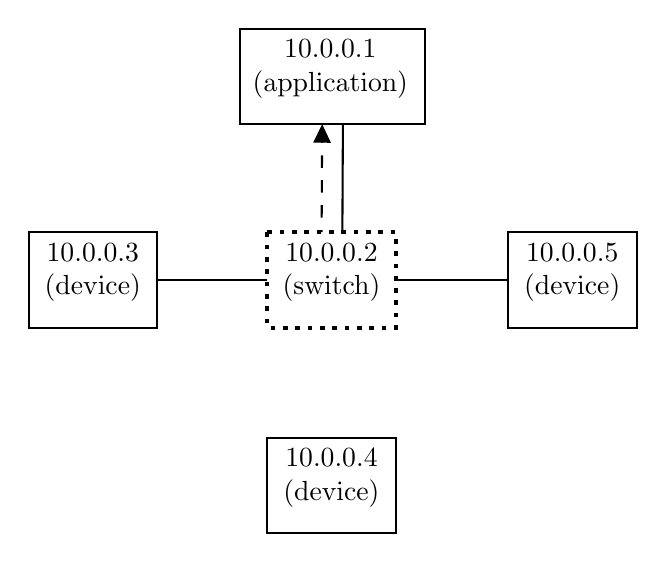
\begin{tikzpicture}[x=0.75pt,y=0.75pt,yscale=-1.0,xscale=1.0]
    %uncomment if require: \path (0,275); %set diagram left start at 0, and has height of 275
    
    
    % Text Node
    \draw    (123,15) -- (212,15) -- (212,61) -- (123,61) -- cycle  ;
    \draw (126,19) node [anchor=north west][inner sep=0.75pt]   [align=left] {\begin{minipage}[lt]{58.25pt}\setlength\topsep{0pt}
    \begin{center}
    10.0.0.1\\(application)
    \end{center}
    
    \end{minipage}};
    % Text Node
    \draw  [dash pattern={on 1.69pt off 2.76pt}][line width=1.5]   (136,113) -- (198,113) -- (198,159) -- (136,159) -- cycle  ;
    \draw (139,117) node [anchor=north west][inner sep=0.75pt]   [align=left] {\begin{minipage}[lt]{39.55pt}\setlength\topsep{0pt}
    \begin{center}
    10.0.0.2\\(switch)
    \end{center}
    
    \end{minipage}};
    % Text Node
    \draw    (21,113) -- (83,113) -- (83,159) -- (21,159) -- cycle  ;
    \draw (24,117) node [anchor=north west][inner sep=0.75pt]   [align=left] {\begin{minipage}[lt]{39.55pt}\setlength\topsep{0pt}
    \begin{center}
    10.0.0.3\\(device)
    \end{center}
    
    \end{minipage}};
    % Text Node
    \draw    (136,212) -- (198,212) -- (198,258) -- (136,258) -- cycle  ;
    \draw (139,216) node [anchor=north west][inner sep=0.75pt]   [align=left] {\begin{minipage}[lt]{39.55pt}\setlength\topsep{0pt}
    \begin{center}
    10.0.0.4\\(device)
    \end{center}
    
    \end{minipage}};
    % Text Node
    \draw    (252,113) -- (314,113) -- (314,159) -- (252,159) -- cycle  ;
    \draw (255,117) node [anchor=north west][inner sep=0.75pt]   [align=left] {\begin{minipage}[lt]{39.55pt}\setlength\topsep{0pt}
    \begin{center}
    10.0.0.5\\(device)
    \end{center}
    
    \end{minipage}};
    % Connection
    \draw    (172.38,61) -- (172.12,113) ;
    % Connection
    \draw    (198,136) -- (252,136) ;
    % Connection
    \draw    (136,136) -- (83,136) ;
    % Connection
    \draw  [dash pattern={on 4.5pt off 4.5pt}]  (162.37,64) -- (162.12,113) ;
    \draw [shift={(162.38,61)}, rotate = 90.29] [fill={rgb, 255:red, 0; green, 0; blue, 0 }  ][line width=0.08]  [draw opacity=0] (8.93,-4.29) -- (0,0) -- (8.93,4.29) -- cycle    ;
\end{tikzpicture}
\end{center}
\caption{Communication is marked as an arrow, scanned devices are highlighted.}
\label{Figure:NetworkDeviceRemove}
\end{figure}


\begin{figure}
\begin{center}
\tikzset{every picture/.style={line width=0.75pt}} %set default line width to 0.75pt        
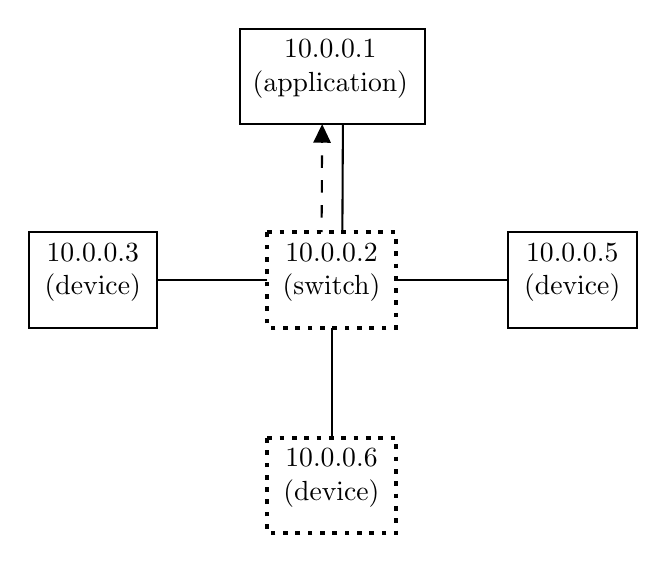
\begin{tikzpicture}[x=0.75pt,y=0.75pt,yscale=-1,xscale=1]
    %uncomment if require: \path (0,278); %set diagram left start at 0, and has height of 278
    % Text Node
    \draw    (122,17) -- (211,17) -- (211,63) -- (122,63) -- cycle  ;
    \draw (125,21) node [anchor=north west][inner sep=0.75pt]   [align=left] {\begin{minipage}[lt]{58.25pt}\setlength\topsep{0pt}
    \begin{center}
    10.0.0.1\\(application)
    \end{center}

    \end{minipage}};
    % Text Node
    \draw  [dash pattern={on 1.69pt off 2.76pt}][line width=1.5]   (135,115) -- (197,115) -- (197,161) -- (135,161) -- cycle  ;
    \draw (138,119) node [anchor=north west][inner sep=0.75pt]   [align=left] {\begin{minipage}[lt]{39.55pt}\setlength\topsep{0pt}
    \begin{center}
    10.0.0.2\\(switch)
    \end{center}

    \end{minipage}};
    % Text Node
    \draw    (20,115) -- (82,115) -- (82,161) -- (20,161) -- cycle  ;
    \draw (23,119) node [anchor=north west][inner sep=0.75pt]   [align=left] {\begin{minipage}[lt]{39.55pt}\setlength\topsep{0pt}
    \begin{center}
    10.0.0.3\\(device)
    \end{center}

    \end{minipage}};
    % Text Node
    \draw  [dash pattern={on 1.69pt off 2.76pt}][line width=1.5]   (135,214) -- (197,214) -- (197,260) -- (135,260) -- cycle  ;
    \draw (138,218) node [anchor=north west][inner sep=0.75pt]   [align=left] {\begin{minipage}[lt]{39.55pt}\setlength\topsep{0pt}
    \begin{center}
    10.0.0.6\\(device)
    \end{center}

    \end{minipage}};
    % Text Node
    \draw    (251,115) -- (313,115) -- (313,161) -- (251,161) -- cycle  ;
    \draw (254,119) node [anchor=north west][inner sep=0.75pt]   [align=left] {\begin{minipage}[lt]{39.55pt}\setlength\topsep{0pt}
    \begin{center}
    10.0.0.5\\(device)
    \end{center}

    \end{minipage}};
    % Connection
    \draw    (171.38,63) -- (171.12,115) ;
    % Connection
    \draw    (197,138) -- (251,138) ;
    % Connection
    \draw    (135,138) -- (82,138) ;
    % Connection
    \draw  [dash pattern={on 4.5pt off 4.5pt}]  (161.37,66) -- (161.12,115) ;
    \draw [shift={(161.38,63)}, rotate = 90.29] [fill={rgb, 255:red, 0; green, 0; blue, 0 }  ][line width=0.08]  [draw opacity=0] (8.93,-4.29) -- (0,0) -- (8.93,4.29) -- cycle    ;
    % Connection
    \draw    (166,161) -- (166,214) ;

\end{tikzpicture}
\end{center}
\caption{Communication is marked as an arrow, scanned devices are highlighted.}
\label{Figure:NetworkDeviceAdded}
\end{figure}

\newpage
\section{How to setup a device}
\label{Section:Evaluation-Setup}

To make a Linux device work with this application, it is necessary to install an LLDP and SNMP daemon and configure them. More detailed information can be found in the man pages of snmpd, lldpd and lldpdcli: \cite{MAN:SNMPD.CONF5:2021} \cite{MAN:LLDPD8:2021} \cite{MAN:LLDPCLI8:2021}. The setup was tested on Debian 10 and may vary depending on the Linux distribution. The first step is to install \textit{lldpd} and \textit{snmpd}. After the installation has been finished, \textit{snmpd} needs to be configured. All configuration needs to be done with superuser permissions. For that, a file needs to be created at \textit{/etc/snmp/snmpd.conf} with the content shown in Listing \ref{Listing:snmpd.conf}.

\begin{lstlisting}[label=Listing:snmpd.conf,captionpos=b,caption={snmpd.conf - Configuration file of the SNMP daemon}]
    # SNMP v3 read-only community "public"
    rouser public noauth
    
    # SNMP v1/v2c read-only community "public"
    rocommunity public
    
    proc 0
    
    # SNMP device info
    syslocation "closet"
    syscontact "Alice"
    sysservices 12
    
    # Activate agentx
    master agentx
\end{lstlisting}

With this configuration, the SNMP daemon will listen to SNMP v1/v2c/V3 requests, when community "public" is used. Entries can only be read and not modified. For SNMPv3 no authentication is needed. The location of the system is "closet", the system administrator is called "Alice" and it should provide information about the system like interface names. It also commands the daemon to activate \textit{agentx}, which allows other daemons like \textit{lldpd} to provide its data over SNMP.

The next step is to configure \textit{lldpd} via the command line interface \textit{lldpcli}. If \textit{lldpcli} is called, a special shell will open. After configuration is finished, the shell can be closed with the command \textit{exit}. The commands needed to configure the LLDP daemon are provided in Listing \ref{Listing:lldpcli}.

\begin{lstlisting}[label=Listing:lldpcli,captionpos=b,caption={Commands to configure lldpd with lldpcli}]
    configure lldp portidsubtype macaddress
    configure system bond-slave-src-mac-type real
    configure lldp capabilities-advertisements
    configure lldp management-addresses-advertisements
    configure lldp agent-type nearest-bridge
\end{lstlisting}

These commands will configure the daemon to publish the MAC address of the port as portid, use the real MAC address of the portadvertise the system capabilities, advertise the management address of the device, and only broadcast the information until the next bridge.

Now both daemons need to be started, for \textit{snmpd} it only needs one command (See Listing \ref{Listing:snmpd}). 
\begin{lstlisting}[language=bash,label=Listing:snmpd,captionpos=b,caption={Starting snmpd.}]
    $ snmpd
\end{lstlisting}

The LLDP daemon, on the other hand, needs to be launched with the \textit{-x} as an argument, this will notify the daemon to search for an agentx and communicate with it. There are two ways to start the daemon, the first way is to start \textit{lldp} directly with the argument (see Listing \ref{Listing:lldpd-x}).
\begin{lstlisting}[label=Listing:lldpd-x,captionpos=b,caption={starting lldpd with agentx support.}]
    $ lldpd -x
\end{lstlisting}

Using the lldp daemon as a service requires a configuration file. This line needs to be added to \textit{/etc/default/lldpd}:
\begin{lstlisting}[language=bash,label=Listing:lldpd-config,captionpos=b,caption={/etc/default/lldpd - Starting the daemon with agent x support.}]
    DAEMON_ARGS="-x"
\end{lstlisting}

\newpage
After adding the line, the daemon can be started with:
\begin{lstlisting}[language=bash,label=Listing:lldpd,captionpos=b,caption={Starting lldpd}]
    $ lldpd
\end{lstlisting}

\section{Requirements}
\label{Section:Evaluation-Requirements}

The application has some requirements to deliver the correct network topology. Every device on the network must fulfill these requirements:

\begin{minipage}{\textwidth}
\begin{itemize}
    \item Run an SNMP daemon.
    \item Support SNMPv1 and SNMPv2c.
    \item Run an LLDP daemon.
    \item LLDP data must be collectible with SNMP.
    \item Each interface port needs to have a unique MAC address.
    \item LLDPd must send the port MAC address as \textit{ChassisID}.
    \item The remote port data must be connected to a local port in the MIB data.
    \item Every network node, that isn't an end node, must send an SNMPv1 trap to the application if the status of an interface changes.
\end{itemize}
\end{minipage}